\documentclass[twoside]{report}


% Load the packagesl

%\usepackage[latin1]{inputenc}
\usepackage[utf8]{inputenc}
%\usepackage[french]{babel}
\usepackage[T1]{fontenc}
\usepackage{amsmath}
%\usepackage{amsfonts}
\usepackage{amssymb} % for the checkmark
\usepackage{makeidx}
\usepackage{graphicx}
\usepackage{lmodern}
\usepackage[left=2.5cm,right=2.5cm,top=2cm,bottom=2cm]{geometry}  % marges
\usepackage{color}
\usepackage{xcolor}
\setcounter{secnumdepth}{4} % augmentation de la num?rotation des sous-sections
\setcounter{tocdepth}{3} % augmentation de la profondeur de la table des mati?res

%\setlength{\parindent}{0cm} %Para las sangrias

% Ce package je ne sais pas pour qu'il soit utilisé
\usepackage{titlesec}

% Ce package est pour plusiers rangées
\usepackage{multirow}

% Ce package est pour la représentation des molécules. Il a besoin de chemist.sty et assurechemist.sty
\usepackage{chemist}

% Ce package est pour la représentation des nombres et des unités de mesure
%\usepackage{si}

\usepackage{svg}

\usepackage{bm}

% Ce package est pour écrire les références avec natbit dans le Harvard style
%\usepackage{natbib}
%\addbibresource{files/bibliographyFile.bib}


% Ce package est pour écrire les références avec biblatex: biblatex.sty, etoolbox.sty, logreq.sty, logreq.def, url.sty
%\usepackage{biblatex}
%\usepackage{cite}
%\addbibresource{bibliographyFile.bib}
%\DeclareNameAlias{sortname}{family-given}
%\DeclareNameAlias{default}{family-given}

% Ce package fait que les phrases ou expressions changent de ligne
\usepackage{makecell}

% Pour les hyperreferences
\usepackage[hidelinks]{hyperref}

% Pour changer l'orientation des foies
\usepackage{pdflscape}
\usepackage{lscape}
%\usepackage[paper=portrait,pagesize]{typearea} % Careful! Changes all the document into portrait mode!

% Pour emphatiser des equations (tables ...)
%\usepackage{empheq}

% Pour changer localement les margins
\usepackage{changepage}

%%%%%%%%%%%%%%%%%%%%%%%%%%%% Pour la bibliographie %%%%%%%%%%%%%%%%%%%%%%%%%%%%%%%

% Bibliographie avec natbib:
\usepackage{natbib}
\bibliographystyle{agsm} %agsm, unsrtnat

\usepackage{subcaption}

%% Bibliographie avec biblatex
%\usepackage[backend=bibtex]{biblatex}
%\addbibresource{files/bibliographyFile.bib}
%\DeclareNameAlias{sortname}{family-given}
%\DeclareNameAlias{default}{family-given}

%%%%%%%%%%%%%%%%%%%%%%%%%%%%%%%%%%%%%%%%%%%%%%%%%%%%%%%%%%%%%%%%%%%%%%%%%%%%%%%%%%
\newcommand{\citepBlackColor}[1][]{({\color{black}\citealt{#1}})}
\newcommand{\citeWhiteColor}[1][]{{\color{white}\cite{#1}}}
\newcommand{\citeColor}[1][]{{\color{blue}\cite{#1}}}
\newcommand{\citepColor}[1][]{({\color{blue}\citealt{#1}})}
\newcommand{\citemColor}[1][]{({\color{blue}\citealt{#1}})}

\newcommand{\introductoryParagraph}[1]{%
\begin{adjustwidth}{1in}{1in}
\textsl{#1}
\end{adjustwidth}
}

\usepackage{gensymb}

\usepackage{fancyhdr}

\usepackage{empheq}
\usepackage{relsize}

\usepackage{upgreek}

% For the diameter symbol
\usepackage{wasysym}

% PACKAGES TO ADD 
%\usepackage{enumitem}   % https://stackoverflow.com/questions/2007627/latex-how-can-i-create-nested-lists-which-look-this-1-1-1-1-1-1-1-2-1-2

\DeclareMathOperator\erf{erf}

%% NOMENCLATURE
% https://www.overleaf.com/learn/latex/nomenclatures
% https://tex.stackexchange.com/questions/112884/how-to-achieve-nomenclature-entries-like-symbol-description-dimension-and-uni
% https://www.youtube.com/watch?v=Ss1XfsaAnfs
% https://tex.stackexchange.com/questions/86666/how-to-create-both-list-of-abbreviations-and-list-of-nomenclature-using-nomencl/87223
\usepackage[intoc]{nomencl}
\makenomenclature

%% this modifies item separation:
\setlength{\nomitemsep}{12pt}

\usepackage{etoolbox}
\renewcommand\nomgroup[1]{%
  \item[\bfseries
  \ifstrequal{#1}{A}{Acronyms}{%
  \ifstrequal{#1}{D}{Dimensionless numbers}{
  \ifstrequal{#1}{G}{Greek Symbols}{%
  \ifstrequal{#1}{R}{Roman Symbols}{%
  \ifstrequal{#1}{Sb}{Subscripts}{%
  \ifstrequal{#1}{Sp}{Superscripts}{}}}}}}%
]}
%]\vspace{10pt}} % this is to add vertical space between the groups.

% This will add the units
%----------------------------------------------
\newcommand{\nomunit}[1]{%
\renewcommand{\nomentryend}{\hspace*{\fill}#1}}
%----------------------------------------------


%%%%% For appendices %%%%%
%\usepackage[toc,page]{appendix}
\usepackage[titletoc]{appendix} % Para apéndices: http://stackoverflow.com/questions/5690679/add-appendix-before-a-in-thesis-toc
\usepackage{chngcntr} %Para los apéndices: http://tex.stackexchange.com/questions/85776/change-figure-numbering-for-appendix

%%%%% Thick lines, ref: https://tex.stackexchange.com/questions/41758/how-can-i-reproduce-this-table-with-thick-lines
\makeatletter
\newcommand{\thickhline}{%
    \noalign {\ifnum 0=`}\fi \hrule height 1pt
    \futurelet \reserved@a \@xhline
}
\newcolumntype{"}{@{\hskip\tabcolsep\vrule width 1pt\hskip\tabcolsep}}
\makeatother


% Redefine paragraph command
\titleformat{\paragraph}
{\normalfont\normalsize\bfseries}{\theparagraph}{1em}{}
\titlespacing*{\paragraph}
{0pt}{3.25ex plus 1ex minus .2ex}{1.5ex plus .2ex}

% Cover: https://tlsflyleaf.onada.fr/
\usepackage[ED=MEGEP-Energ,Ets=INP]{tlsflyleaf}

% For highlighting
\usepackage{color,soul}


% Create commands
%\newcommand{\tab_space}{[0.3cm]}
\def \tab_space {\\[0.2cm]}

% 
\usepackage{array,booktabs}


% Greek letters inkscape:
% http://kestrel.nmt.edu/~raymond/software/howtos/greekscape.xhtml

% Headers and footers
\renewcommand{\chaptermark}[1]{\markboth{\chaptername\ \thechapter.\ #1}{}}
\renewcommand{\sectionmark}[1]{\markright{\thesection.\ #1}}

\pagestyle{fancy}
\fancyhead[LE]{\leftmark}
\fancyhead[RE]{}
\fancyhead[LO]{}
%\fancyhead[RO]{Guides and tutorials}
\fancyfoot[CE,CO]{\thepage}



% volume fraction reference in document:
% \ref{eq:vol_frac_definition}

\begin{document}


\begin{figure}[h!]
\flushleft
\begin{subfigure}[b]{0.2\textwidth}
	\flushleft
%	\hspace*{-0.35in}
   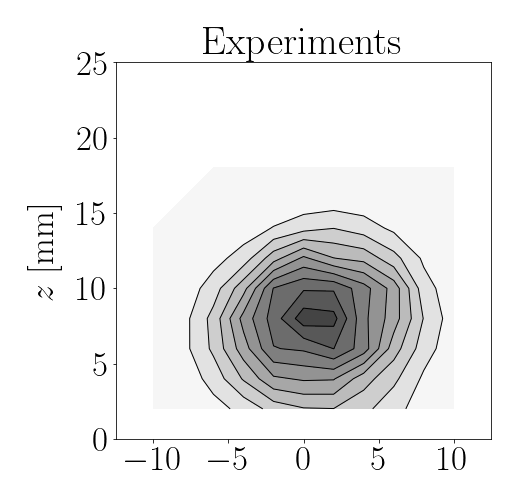
\includegraphics[scale=0.4]{./part2_developments/figures_ch6_lagrangian_JICF/params_breakup_model/maps/expe_flux}
   %\label{} 
\end{subfigure}
\hspace*{0.27in}
\begin{subfigure}[b]{0.2\textwidth}
	\flushleft
   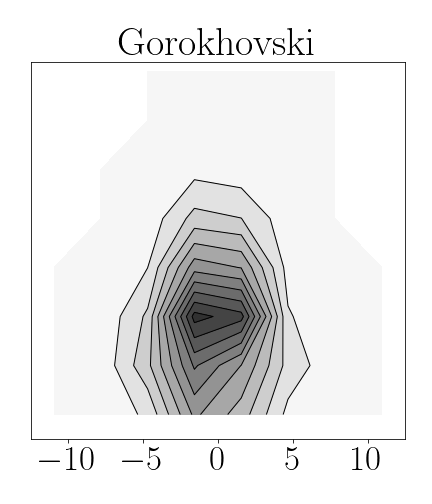
\includegraphics[scale=0.4]{./part2_developments/figures_ch6_lagrangian_JICF/params_breakup_model/maps/goro_flux}
   %\label{} 
\end{subfigure}
\hspace*{0.02in}
\begin{subfigure}[b]{0.2\textwidth}
	\flushleft
   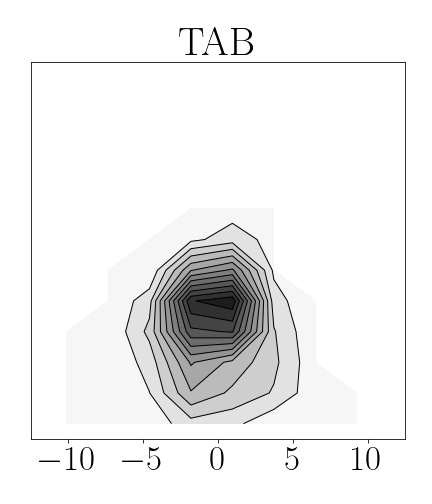
\includegraphics[scale=0.4]{./part2_developments/figures_ch6_lagrangian_JICF/params_breakup_model/maps/TAB_flux}
   %\label{} 
\end{subfigure}
\hspace*{0.02in}
\begin{subfigure}[b]{0.2\textwidth}
	\flushleft
   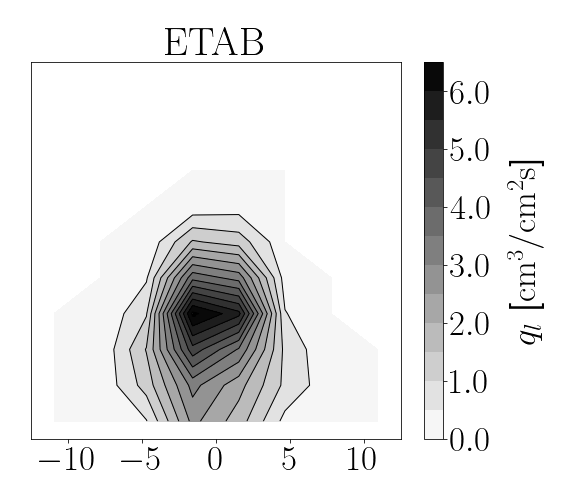
\includegraphics[scale=0.4]{./part2_developments/figures_ch6_lagrangian_JICF/params_breakup_model/maps/ETAB_flux}
   %\label{} 
\end{subfigure}

\vspace*{-0.25in}

\flushleft
\begin{subfigure}[b]{0.2\textwidth}
	\flushleft
%	\hspace*{-0.35in}
   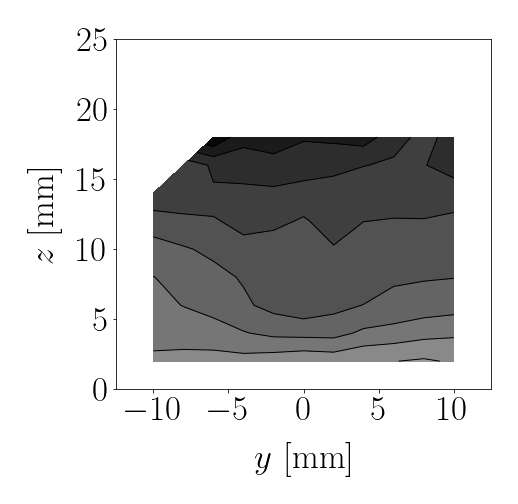
\includegraphics[scale=0.4]{./part2_developments/figures_ch6_lagrangian_JICF/params_breakup_model/maps/expe_SMD}
   %\label{} 
\end{subfigure}
\hspace*{0.27in}
\begin{subfigure}[b]{0.2\textwidth}
	\flushleft
   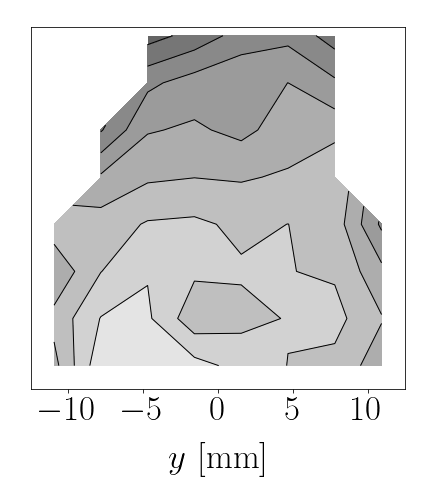
\includegraphics[scale=0.4]{./part2_developments/figures_ch6_lagrangian_JICF/params_breakup_model/maps/goro_SMD}
   %\label{} 
\end{subfigure}
\hspace*{0.02in}
\begin{subfigure}[b]{0.2\textwidth}
	\flushleft
   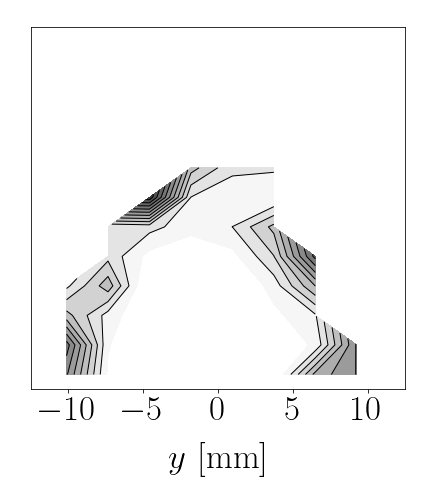
\includegraphics[scale=0.4]{./part2_developments/figures_ch6_lagrangian_JICF/params_breakup_model/maps/TAB_SMD}
   %\label{} 
\end{subfigure}
\hspace*{0.02in}
\begin{subfigure}[b]{0.2\textwidth}
	\flushleft
   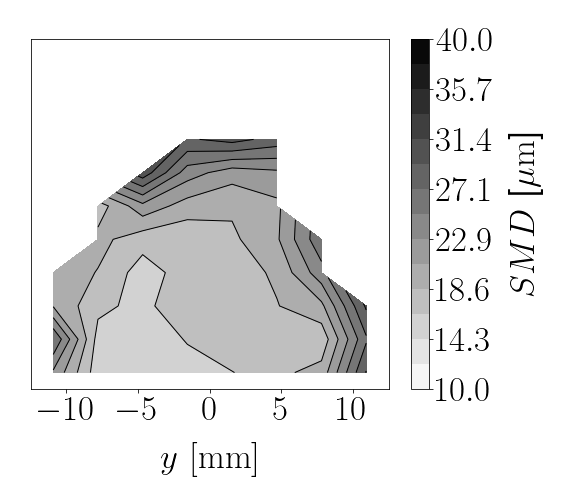
\includegraphics[scale=0.4]{./part2_developments/figures_ch6_lagrangian_JICF/params_breakup_model/maps/ETAB_SMD}
   %\label{} 
\end{subfigure}



\caption{Flux and SMD maps for numerical simulations comparing the effect of calibrating the constants from the Gorokhovski model with the experimental results}
\label{fig:maps_LGS_JICF_second_atom_apte_calibration}
\end{figure}







\end{document}